\section{提案手法: Basket-aware Apriori-Window}
\label{sec:proposed_method}

%% ====== 4.1 従来法の問題の形式的説明 ======
\subsection{従来法（flatten）の問題}
\label{sec:conventional_problem}

従来の Apriori-window~\cite{dsaa2025} はバスケット構造を扱う設計になっていないため，
バスケット構造付きトランザクションデータに適用する際には，
各トランザクションの全バスケットを統合（flatten）して単一アイテムセットに
変換する前処理が必要である．

\begin{definition}[フラット化]
\label{def:flatten}
バスケット構造付きトランザクション $d = (ts, \mathcal{B})$ の
\emph{フラット化}（flatten）とは，全バスケットの和集合を計算し，
$d_{\text{flat}} = (ts, \bigcup_{B \in \mathcal{B}} B)$ という
単一アイテムセットのトランザクションを生成することである．
\end{definition}

フラット化後のトランザクションデータに Apriori-window を適用することで，
トランザクション内サポート（式~(\ref{eq:txn_support})）に基づく
密集パターンが抽出される．このとき，命題~\ref{prop:monotone} より
$\text{txn\_support}(P) \geq \text{true\_support}(P)$ であるため，
従来法は真の密集パターンに加えて偽共起パターンも検出してしまう（定義~\ref{def:spurious}）．

\begin{figure}[t]
    \centering
    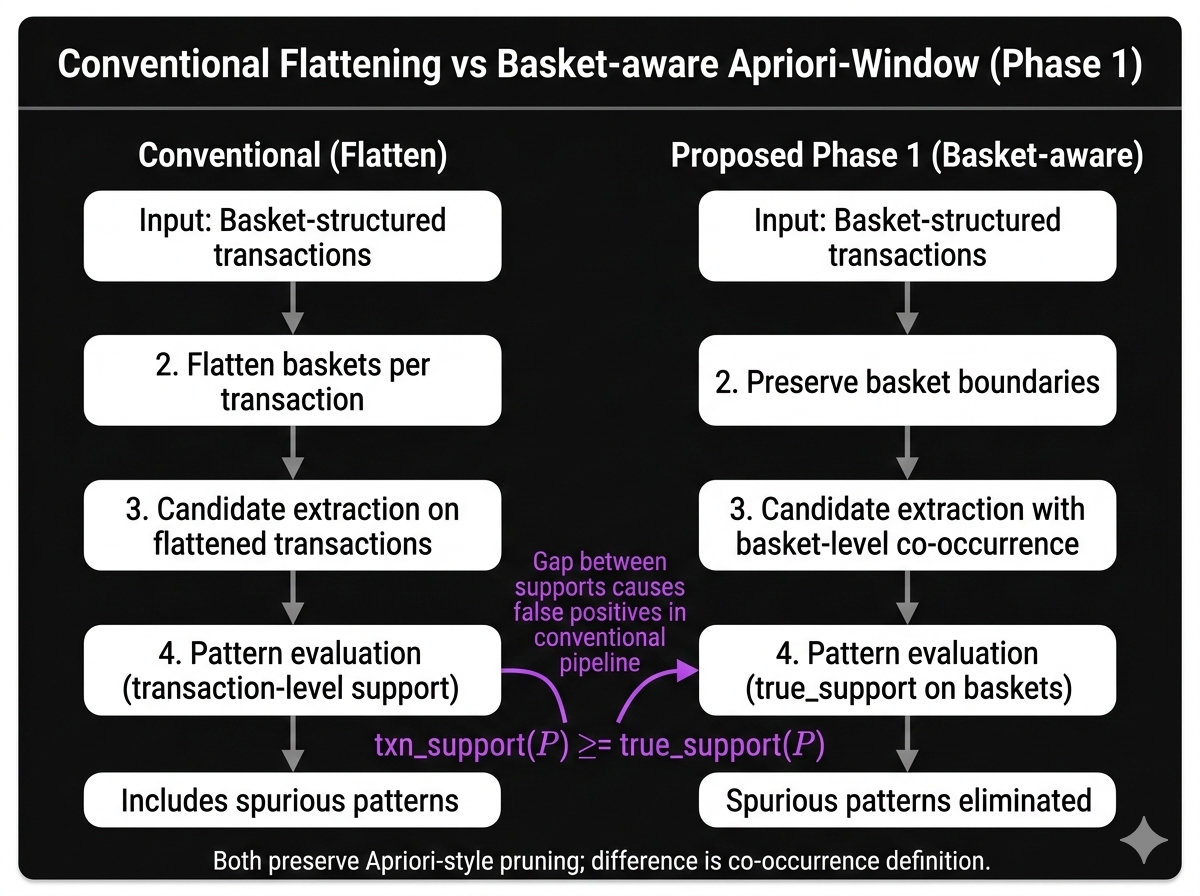
\includegraphics[width=\linewidth]{fig/conventional_vs_phase1.png}
    \caption{従来法（flatten）と提案手法の処理比較}
    \label{fig:conventional_vs_phase1}
\end{figure}

図~\ref{fig:conventional_vs_phase1} は，従来法がバスケットを統合して
トランザクション内共起を数えるのに対し，提案法がバスケット境界を維持して
共起を評価する差分を示している．

%% ====== 4.2 アルゴリズムの概要 ======
\subsection{アルゴリズム概要}
\label{sec:algorithm}

提案手法 \emph{Basket-aware Apriori-Window}は，
バスケット内共起（定義~\ref{def:intra_basket}）のみに基づいてサポートを計算することで，
原理的に偽共起パターンを出力しない．
アルゴリズム~\ref{alg:basket_aware_apriori_window} に全体の手順を示す．

\begin{algorithm}[t]
\caption{Basket-aware Apriori-Window}
\label{alg:basket_aware_apriori_window}
\begin{algorithmic}[1]
\Require バスケット構造付きトランザクションデータ $D$，
         最小サポート $\theta$，最小区間長 $W$，最大長 $L$
\Ensure  バスケット対応密集パターンとその密集区間の集合 $\mathcal{F}$

\State $\mathcal{F} \leftarrow \emptyset$
\State \Comment{--- ステップ 1: バスケットマップの構築 ---}
\State $(M_{\text{item}},\, \text{b2t},\, M_{\text{txn}})
       \leftarrow \Call{BuildBasketMap}{D}$
\State \Comment{$M_{\text{item}}[i]$: アイテム $i$ が含まれるバスケット ID のリスト}
\State \Comment{$\text{b2t}[b]$: バスケット $b$ が属するトランザクション ID}
\State \Comment{$M_{\text{txn}}[i]$: アイテム $i$ が含まれるトランザクション ID のリスト}

\State \Comment{--- ステップ 2: 長さ 1 の密集パターン ---}
\State $\mathcal{F}_1 \leftarrow \emptyset$
\For{each item $i \in \mathcal{I}$}
    \State $\text{intervals} \leftarrow
        \Call{SlidingWindow}{M_{\text{txn}}[i],\, \theta,\, W}$
    \If{$\text{intervals} \neq \emptyset$}
        \State $\mathcal{F}_1 \leftarrow \mathcal{F}_1 \cup \{(\{i\},\, \text{intervals})\}$
    \EndIf
\EndFor
\State $\mathcal{F} \leftarrow \mathcal{F} \cup \mathcal{F}_1$

\State \Comment{--- ステップ 3: 長さ $k \geq 2$ の密集パターン ---}
\State $k \leftarrow 2$
\While{$\mathcal{F}_{k-1} \neq \emptyset$ \textbf{and} $k \leq L$}
    \State $\mathcal{C}_k \leftarrow
        \Call{GenerateCandidates}{\mathcal{F}_{k-1}}$
    \State \Comment{Apriori 反単調性による枝刈り済み候補集合}
    \State $\mathcal{F}_k \leftarrow \emptyset$
    \For{each candidate $P \in \mathcal{C}_k$}
        \State \Comment{\textbf{Key: バスケットレベルの共起集合を計算}}
        \State $B_P \leftarrow \bigcap_{i \in P} M_{\text{item}}[i]$
        \State \Comment{$B_P$: $P$ の全アイテムを同時に含むバスケット ID の集合}
        \State $T_P \leftarrow \Call{BasketToTransaction}{B_P,\, \text{b2t}}$
        \State \Comment{$T_P$: $B_P$ に対応するトランザクション ID のリスト}
        \State $\text{intervals} \leftarrow
            \Call{SlidingWindow}{T_P,\, \theta,\, W}$
        \If{$\text{intervals} \neq \emptyset$}
            \State $\mathcal{F}_k \leftarrow
                \mathcal{F}_k \cup \{(P,\, \text{intervals})\}$
        \EndIf
    \EndFor
    \State $\mathcal{F} \leftarrow \mathcal{F} \cup \mathcal{F}_k$
    \State $k \leftarrow k + 1$
\EndWhile

\State \Return $\mathcal{F}$
\end{algorithmic}
\end{algorithm}


\subsubsection{ステップ 1: バスケットマップの構築}

$\Call{BuildBasketMap}{}$ は，データ全体を 1 回走査して 3 つのデータ構造を構築する．

\begin{itemize}
    \item $M_{\text{item}}[i]$（アイテム→バスケット ID マップ）:
    アイテム $i$ が含まれるバスケットのグローバル ID のリスト（昇順ソート済み）．
    同一バスケット内に同じアイテムが複数あっても 1 回のみ記録する．

    \item $\text{b2t}[b]$（バスケット→トランザクション ID マップ）:
    バスケット $b$ が属するトランザクションのインデックス．
    トランザクション順 × バスケット順でグローバル連番を付与するため，
    この配列は単調非減少となる．

    \item $M_{\text{txn}}[i]$（アイテム→トランザクション ID マップ）:
    アイテム $i$ が（いずれかのバスケットに）含まれるトランザクションのインデックスのリスト
    （重複なし・昇順）．長さ 1 パターンのスライディングウィンドウ処理で使用する．
\end{itemize}

\subsubsection{ステップ 2: 長さ 1 の密集パターン}

各単体アイテム $i$ に対して，$M_{\text{txn}}[i]$（アイテムの出現トランザクション ID 列）
を入力としてスライディングウィンドウ機構を実行し，
$\text{true\_support}_I(i) \geq \theta$ かつ $n(D_I) \geq W$ を満たす
すべての密集区間を求める．長さ 1 のアイテムについては，
バスケット内共起とトランザクション内共起が一致する（1 アイテムは常に単一バスケット内）
ため，この処理は従来法と等価である．

\subsubsection{ステップ 3: 長さ $k \geq 2$ の密集パターン（核心部）}

アルゴリズム~\ref{alg:basket_aware_apriori_window} の 21〜27 行目が本手法の核心部である．
候補アイテムセット $P$ に対して，バスケット ID の集合積
$B_P = \bigcap_{i \in P} M_{\text{item}}[i]$ を計算する．
$B_P$ は $P$ のすべてのアイテムを同時に含むバスケットの集合であり，
\emph{バスケット内共起を直接エンコードする}．

続いて，$B_P$ を $\text{b2t}$ を用いてトランザクション ID 列 $T_P$ に変換し
（$\Call{BasketToTransaction}{}$），スライディングウィンドウを適用して密集区間を求める．

\textbf{従来法との違い}: 従来法では，候補 $P$ のサポートを計算するために
$T_P = \bigcap_{i \in P} M_{\text{txn}}[i]$ というトランザクション ID の集合積を用いる．
これは，各アイテムがそのトランザクションのいずれかのバスケットに存在することを確認するだけで，
同一バスケット内の共起は保証しない．提案手法は集合積をバスケット粒度で行うことで，
この問題を根本的に解決する．

\subsubsection{スライディングウィンドウ機構}

$\Call{SlidingWindow}{}$ の実装は先行研究 Apriori-window~\cite{dsaa2025} と同一である．
固定幅 $W$ のウィンドウを 1 トランザクション単位でスライドさせながら，
ウィンドウ内のサポートが $\theta$ を超える区間を記録し，
隣接区間を統合して密集区間リストを返す．また，ウィンドウ内でサポートが $\theta$ を
大幅に上回る場合には，余剰分に基づいてストライドを増加させる最適化（stride adjustment）
を適用して効率的な走査を実現する~\cite{dsaa2025}．

%% ====== 4.3 反単調性の証明 ======
\subsection{反単調性の証明}
\label{sec:anti_monotone}

Apriori の枝刈りが機能するためには，候補のサポートが単調非増加（反単調性）で
あることが必要である．従来の Apriori-window では定義域をトランザクション単位の
出現集合としてこれを証明しているが~\cite{dsaa2025}，
提案手法ではバスケット粒度での反単調性を証明する必要がある．

\begin{theorem}[バスケット内共起における反単調性]
\label{thm:anti_monotone}
任意のアイテムセット $P$ とその真の上位集合 $P' \supset P$，
任意の区間 $I$ に対して，
\begin{equation}
\text{true\_support}_I(P') \leq \text{true\_support}_I(P)
\label{eq:anti_monotone}
\end{equation}
が成立する．
\end{theorem}

\begin{proof}
$d = (ts, \mathcal{B})$ を区間 $I$ 内の任意のトランザクションとする．

$P'$ がバスケット内共起する（$\exists B \in \mathcal{B}: P' \subseteq B$）ならば，
$P \subset P'$ より $P \subseteq B$ も成立するため，
$P$ もそのバスケット $B$ でバスケット内共起する．

逆は一般に成立しない（$P$ がバスケット内共起しても，$P'$ の余分なアイテムが
同一バスケットに含まれるとは限らない）．

したがって，$P'$ がバスケット内共起するトランザクションの集合は，
$P$ がバスケット内共起するトランザクションの集合の部分集合であり，
式~(\ref{eq:anti_monotone}) が成立する．
\end{proof}

定理~\ref{thm:anti_monotone} より，あるアイテムセット $P$ が
バスケット対応密集パターンでない（すなわち，すべての区間 $I$ で
$\text{true\_support}_I(P) < \theta$ または $n(D_I) < W$）ならば，
$P$ の任意の上位集合 $P'$ もバスケット対応密集パターンにならない．
これにより，$\Call{GenerateCandidates}{}$（$\mathcal{F}_{k-1}$ に含まれない
パターンを部分集合にもつ候補を除外する Apriori 枝刈り）の正当性が保証される．

%% ====== 4.4 計算量解析 ======
\subsection{計算量解析}
\label{sec:complexity}

\begin{theorem}[時間計算量]
\label{thm:complexity}
$N$ をトランザクション数，$B_{\text{total}}$ を全バスケット数，
$m$ をアイテム数，$L$ を最大アイテムセット長，
$\bar{b}$ をアイテムあたりの平均出現バスケット数とする．
Basket-aware Apriori-Window の時間計算量は
\begin{equation}
O\bigl(B_{\text{total}} \cdot \bar{K} + \sum_{k=1}^{L} |\mathcal{C}_k| \cdot k \cdot \bar{b} + \sum_{k=1}^{L} |\mathcal{C}_k| \cdot N\bigr)
\end{equation}
である．ここで $\bar{K}$ はバスケットあたりの平均アイテム数である．
第 1 項はバスケットマップ構築，第 2 項はバスケット ID の集合積，
第 3 項はスライディングウィンドウ走査に対応する．
\end{theorem}

\begin{proof}
\textbf{ステップ 1}（バスケットマップ構築）:
全バスケットを 1 回走査し，各アイテムを $M_{\text{item}}$ と $M_{\text{txn}}$ に登録する．
走査コストは $\sum_{b} |b| = B_{\text{total}} \cdot \bar{K}$ である．

\textbf{ステップ 2}（長さ 1）:
$m$ 個のアイテムそれぞれに対してスライディングウィンドウを実行する．
各ウィンドウ走査は $O(N)$ であり，合計 $O(m \cdot N)$ である．

\textbf{ステップ 3}（長さ $k \geq 2$）:
各候補 $P \in \mathcal{C}_k$ に対して，
$k$ 個のバスケット ID リストの集合積を計算する．
ソート済みリストのマージにより $O(k \cdot \bar{b})$ である．
続くスライディングウィンドウは $O(N)$ である．
候補数 $|\mathcal{C}_k|$ は Apriori 枝刈りにより
$\binom{|\mathcal{F}_{k-1}|}{2}$ 以下に抑えられる．
\end{proof}

\begin{proposition}[空間計算量]
\label{prop:space}
$M_{\text{item}}$ の総サイズは $O(B_{\text{total}} \cdot \bar{K})$，
$\text{b2t}$ は $O(B_{\text{total}})$，
$M_{\text{txn}}$ は $O(N \cdot \bar{K}_{\text{txn}})$
（$\bar{K}_{\text{txn}}$: トランザクションあたりの平均ユニークアイテム数）である．
従来法の $M_{\text{txn}}$ のみの保持に対して，
追加空間は $M_{\text{item}}$ と $\text{b2t}$ の $O(B_{\text{total}} \cdot (\bar{K}+1))$ である．
\end{proposition}

%% ====== 4.5 従来 Apriori-window との関係 ======
\subsection{従来 Apriori-window との関係}
\label{sec:relationship}

\begin{proposition}[特殊ケースとしての従来法]
\label{prop:special_case}
各トランザクションがちょうど 1 つのバスケット（$|\mathcal{B}| = 1$）をもつとき，
提案手法の出力は従来 Apriori-window の出力と一致する．
\end{proposition}

\begin{proof}
$|\mathcal{B}| = 1$ の場合，バスケット内共起とトランザクション内共起は
同値であるため（$\exists B \in \mathcal{B}: P \subseteq B$
$\Leftrightarrow$ $P \subseteq \bigcup_{B \in \mathcal{B}} B$），
$\text{true\_support}_I(P) = \text{txn\_support}_I(P)$ が成立する．
したがって，提案手法と従来法は同一の密集パターンを出力する．
\end{proof}

命題~\ref{prop:special_case} は，提案手法が従来 Apriori-window の
\emph{上位互換（strict generalization）}であることを示す．
すなわち，従来法は $\lambda_{\text{baskets}} = 1$（各トランザクションに
バスケットが 1 つしかない場合）の特殊ケースとして包含される．

%% ====== 4.5 実装上のポイント ======
\subsection{実装上のポイント}

\subsubsection{BasketToTransaction におけるトランザクション ID の重複}
$\Call{BasketToTransaction}{}$ は，バスケット ID リスト $B_P$ を
対応するトランザクション ID 列 $T_P$ に変換する．
ここで，$B_P$ に同一トランザクションの複数バスケット
$b_1, b_2$ が含まれる（$\text{b2t}[b_1] = \text{b2t}[b_2] = t$）場合，
トランザクション $t$ は $T_P$ に \emph{1 回のみ} 記録される設計とする．

これは，$\text{true\_support}$ の定義（式~(\ref{eq:true_support})）が
トランザクション単位でカウントを行うことに対応している．
すなわち，1 つのトランザクション内に $P$ を含むバスケットが複数あっても，
サポートへの貢献は 1 とみなす．

\subsubsection{グローバルバスケット ID の採番}
バスケット ID はトランザクション順 × バスケット順にグローバル連番を付与する．
この採番規則により，$\text{b2t}$ 配列が単調非減少となり，
ソート済みリストとの二分探索による高速な集合積計算（バスケット ID の積集合）が
$O(|B_{P_1}| + |B_{P_2}|)$（$P = \{i_1, i_2\}$ の場合のマージ）で可能になる．

\subsubsection{メモリ効率}
長さ 1 の密集パターンのみに関与する単体アイテムについては，
$M_{\text{item}}[i]$ は長さ 1 パターンの密集区間計算後に解放可能である．
ただし，長さ 2 以上の候補生成時には再び必要になるため，
全プロセスを通じて保持する実装が現実的である．
